%%%% Paramétrage du TD %%%%
\def\xxactivite{Application 01 \ifprof -- Corrigé \else \fi }
\def\xxauteur{\textsl{Xavier Pessoles}}


\def\xxnumchapitre{Révisions 2 \vspace{.2cm}}
\def\xxchapitre{\hspace{.12cm} Modéliser les systèmes asservis -- Transformée de Laplace}

\def\xxcompetences{%
\textsl{%
\textbf{Savoirs et compétences :}\\
\vspace{-.4cm}
\begin{itemize}[label=\ding{112},font=\color{ocre}] 
%\item \textit{Mod3.C2 : } pôles dominants et réduction de l’ordre du modèle : principe, justification
%\item \textit{Res2.C4 : } stabilité des SLCI : définition entrée bornée -- sortie bornée (EB -- SB)	
%\item \textit{Res2.C5 : } stabilité des SLCI : équation caractéristique	
%\item \textit{Res2.C6 : } stabilité des SLCI : position des pôles dans le plan complexe
\item ...%\textit{Res2.C7 : } stabilité des SLCI : marges de stabilité (de gain et de phase)
\end{itemize}
}}


\def\xxfigures{
%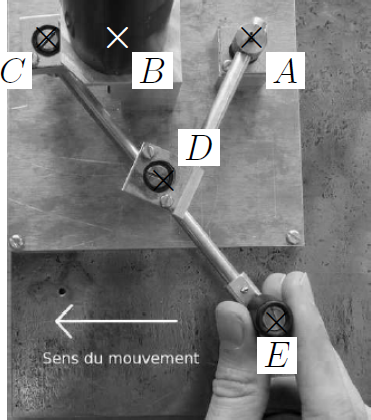
\includegraphics[width=.9\linewidth]{fig_00}
}%figures de la page de garde

\def\xxtitreexo{Application}
\def\xxsourceexo{}

\iflivret
\pagestyle{empty}


%%%%%%%% PAGE DE GARDE COURS
\ifcours
% ==== BANDEAU DES TITRES ==== 
\begin{tikzpicture}[remember picture,overlay]
\node at (current page.north west)
{\begin{tikzpicture}[remember picture,overlay]
\node[anchor=north west,inner sep=0pt] at (0,0) {\includegraphics[width=\paperwidth]{\thechapterimage}};
\draw[anchor=west] (-2cm,-8cm) node [line width=2pt,rounded corners=15pt,draw=ocre,fill=white,fill opacity=0.6,inner sep=40pt]{\strut\makebox[22cm]{}};
\draw[anchor=west] (1cm,-8cm) node {\huge\sffamily\bfseries\color{black} %
\begin{minipage}{1cm}
\rotatebox{90}{\LARGE\sffamily\textsc{\color{ocre}\textbf{\xxnumpartie}}}
\end{minipage} \hfill
\begin{minipage}[c]{14cm}
\begin{titrepartie}
\begin{flushright}
\renewcommand{\baselinestretch}{1.1} 
\Large\sffamily\textsc{\textbf{\xxpartie}}
\renewcommand{\baselinestretch}{1} 
\end{flushright}
\end{titrepartie}
\end{minipage} \hfill
\begin{minipage}[c]{3.5cm}
{\large\sffamily\textsc{\textbf{\color{ocre} \discipline}}}
\end{minipage} 
 };
\end{tikzpicture}};
\end{tikzpicture}
% ==== FIN BANDEAU DES TITRES ==== 


% ==== ONGLET 
\begin{tikzpicture}[overlay]
\node[shape=rectangle, 
      rounded corners = .25 cm,
	  draw= ocre,
	  line width=2pt, 
	  fill = ocre!10,
	  minimum width  = 2.5cm,
	  minimum height = 3cm,] at (18.3cm,0) {};
\node at (17.7cm,0) {\rotatebox{90}{\textbf{\Large\color{ocre}{\classe}}}};
%{};
\end{tikzpicture}
% ==== FIN ONGLET 


\vspace{3.5cm}

\begin{tikzpicture}[remember picture,overlay]
\draw[anchor=west] (-2cm,-6cm) node {\huge\sffamily\bfseries\color{black} %
\begin{minipage}{2cm}
\begin{center}
\LARGE\sffamily\textsc{\color{ocre}\textbf{\xxactivite}}
\end{center}
\end{minipage} \hfill
\begin{minipage}[c]{15cm}
\begin{titrechapitre}
\renewcommand{\baselinestretch}{1.1} 
\Large\sffamily\textsc{\textbf{\xxnumchapitre}}

\Large\sffamily\textsc{\textbf{\xxchapitre}}
\vspace{.5cm}

\renewcommand{\baselinestretch}{1} 
\normalsize\normalfont
\xxcompetences
\end{titrechapitre}
\end{minipage}  };
\end{tikzpicture}
\vfill

\begin{flushright}
\begin{minipage}[c]{.3\linewidth}
\begin{center}
\xxfigures
\end{center}
\end{minipage}\hfill
\begin{minipage}[c]{.6\linewidth}
\startcontents
%\printcontents{}{1}{}
\printcontents{}{1}{}
\end{minipage}
\end{flushright}

\begin{tikzpicture}[remember picture,overlay]
\draw[anchor=west] (4.5cm,-.7cm) node {
\begin{minipage}[c]{.2\linewidth}
\begin{flushright}

\includegraphics[width=2cm]{logoCC}
\end{flushright}
\end{minipage}
\begin{minipage}[c]{.2\linewidth}
\textsl{\xxauteur} \\
\textsl{\classe}
\end{minipage}
 };
\end{tikzpicture}

\newpage
\pagestyle{fancy}

%\newpage
%\pagestyle{fancy}

\else
\fi
%% FIN PAGE DE GARDE DES COURS

%%%%%%%% PAGE DE GARDE TD
\iftd

% BANDEAU EXO
\iflivret % SI LIVRET
\begin{tikzpicture}[remember picture,overlay]
\draw[anchor=west] (-2cm,-3.3cm) node {\huge\sffamily\bfseries\color{black} %
\begin{minipage}{5cm}
\begin{center}
\LARGE\sffamily\color{ocre}\textbf{\textsc{\xxactivite}}

\begin{center}
\xxfigures
\end{center}

\end{center}
\end{minipage} \hfill
\begin{minipage}[c]{12cm}
\begin{titrechapitre}
\renewcommand{\baselinestretch}{1.1} 
\large\sffamily\textbf{\textsc{\xxtitreexo}}

\small\sffamily{\textbf{\textit{\color{black!70}\xxsourceexo}}}
\vspace{.5cm}

\renewcommand{\baselinestretch}{1} 
\normalsize\normalfont
\xxcompetences
\end{titrechapitre}
\end{minipage}};
\end{tikzpicture}
\else % ELSE NOT LIVRET
\begin{tikzpicture}[remember picture,overlay]
\draw[anchor=west] (-2cm,-4.5cm) node {\huge\sffamily\bfseries\color{black} %
\begin{minipage}{5cm}
\begin{center}
\LARGE\sffamily\color{ocre}\textbf{\textsc{\xxactivite}}

\begin{center}
\xxfigures
\end{center}

\end{center}
\end{minipage} \hfill
\begin{minipage}[c]{12cm}
\begin{titrechapitre}
\renewcommand{\baselinestretch}{1.1} 
\large\sffamily\textbf{\textsc{\xxtitreexo}}

\small\sffamily{\textbf{\textit{\color{black!70}\xxsourceexo}}}
\vspace{.5cm}

\renewcommand{\baselinestretch}{1} 
\normalsize\normalfont
\xxcompetences
\end{titrechapitre}
\end{minipage}};
\end{tikzpicture}

\fi

\else   % FIN IF TD
\fi


%%%%%%%% PAGE DE GARDE FICHE
\iffiche
\begin{tikzpicture}[remember picture,overlay]
\node at (current page.north west)
{\begin{tikzpicture}[remember picture,overlay]
\draw[anchor=west] (-2cm,-2.25cm) node [line width=2pt,rounded corners=15pt,draw=ocre,fill=white,fill opacity=0.6,inner sep=40pt]{\strut\makebox[22cm]{}};
\draw[anchor=west] (1cm,-2.25cm) node {\huge\sffamily\bfseries\color{black} %
\begin{minipage}{1cm}
\rotatebox{90}{\LARGE\sffamily\textsc{\color{ocre}\textbf{\xxnumpartie}}}
\end{minipage} \hfill
\begin{minipage}[c]{14cm}
\begin{titrepartie}
\begin{flushright}
\renewcommand{\baselinestretch}{1.1} 
\large\sffamily\textsc{\textbf{\xxpartie} \\} 

\vspace{.2cm}

\normalsize\sffamily\textsc{\textbf{\xxnumchapitre -- \xxchapitre}}
\renewcommand{\baselinestretch}{1} 
\end{flushright}
\end{titrepartie}
\end{minipage} \hfill
\begin{minipage}[c]{3.5cm}
{\large\sffamily\textsc{\textbf{\color{ocre} \discipline}}}
\end{minipage} 
 };
\end{tikzpicture}};
\end{tikzpicture}

\iflivret % SI LIVRET
\begin{tikzpicture}[overlay]
\node[shape=rectangle, 
      rounded corners = .25 cm,
	  draw= ocre,
	  line width=2pt, 
	  fill = ocre!10,
	  minimum width  = 2.5cm,
	  minimum height = 2.5cm,] at (18.5cm,.5cm) {};
\node at (17.9cm,.5cm) {\rotatebox{90}{\textsf{\textbf{\large\color{ocre}{\classe}}}}};
%{};
\end{tikzpicture}
\else  % SI PAS LIVRET
\iftd %% SI TD et PAS LIVRET
\begin{tikzpicture}[overlay]
\node[shape=rectangle, 
      rounded corners = .25 cm,
	  draw= ocre,
	  line width=2pt, 
	  fill = ocre!10,
	  minimum width  = 2.5cm,
	  minimum height = 2.5cm,] at (18.6cm,0.9cm) {};
\node at (18cm,0.9cm) {\rotatebox{90}{\textsf{\textbf{\large\color{ocre}{\classe}}}}};
%{};
\end{tikzpicture}

\else % FIN DU SI TD PAS LIVRET 
\begin{tikzpicture}[overlay]
\node[shape=rectangle, 
      rounded corners = .25 cm,
	  draw= ocre,
	  line width=2pt, 
	  fill = ocre!10,
	  minimum width  = 2.5cm,
%	  minimum height = 2.5cm,] at (18.5cm,1.1cm) {};
	  minimum height = 2.5cm,] at (18.6cm,0.5cm) {};
\node at (18cm,0.5cm) {\rotatebox{90}{\textsf{\textbf{\large\color{ocre}{\classe}}}}};
%{};
\end{tikzpicture}
\fi
\fi
\else
\fi



\else
\pagestyle{empty}


%%%%%%%% PAGE DE GARDE COURS
\ifcours
% ==== BANDEAU DES TITRES ==== 
\begin{tikzpicture}[remember picture,overlay]
\node at (current page.north west)
{\begin{tikzpicture}[remember picture,overlay]
\node[anchor=north west,inner sep=0pt] at (0,0) {\includegraphics[width=\paperwidth]{\thechapterimage}};
\draw[anchor=west] (-2cm,-8cm) node [line width=2pt,rounded corners=15pt,draw=ocre,fill=white,fill opacity=0.6,inner sep=40pt]{\strut\makebox[22cm]{}};
\draw[anchor=west] (1cm,-8cm) node {\huge\sffamily\bfseries\color{black} %
\begin{minipage}{1cm}
\rotatebox{90}{\LARGE\sffamily\textsc{\color{ocre}\textbf{\xxnumpartie}}}
\end{minipage} \hfill
\begin{minipage}[c]{14cm}
\begin{titrepartie}
\begin{flushright}
\renewcommand{\baselinestretch}{1.1} 
\Large\sffamily\textsc{\textbf{\xxpartie}}
\renewcommand{\baselinestretch}{1} 
\end{flushright}
\end{titrepartie}
\end{minipage} \hfill
\begin{minipage}[c]{3.5cm}
{\large\sffamily\textsc{\textbf{\color{ocre} \discipline}}}
\end{minipage} 
 };
\end{tikzpicture}};
\end{tikzpicture}
% ==== FIN BANDEAU DES TITRES ==== 


% ==== ONGLET 
\begin{tikzpicture}[overlay]
\node[shape=rectangle, 
      rounded corners = .25 cm,
	  draw= ocre,
	  line width=2pt, 
	  fill = ocre!10,
	  minimum width  = 2.5cm,
	  minimum height = 3cm,] at (18.3cm,0) {};
\node at (17.7cm,0) {\rotatebox{90}{\textbf{\Large\color{ocre}{\classe}}}};
%{};
\end{tikzpicture}
% ==== FIN ONGLET 


\vspace{3.5cm}

\begin{tikzpicture}[remember picture,overlay]
\draw[anchor=west] (-2cm,-6cm) node {\huge\sffamily\bfseries\color{black} %
\begin{minipage}{2cm}
\begin{center}
\LARGE\sffamily\textsc{\color{ocre}\textbf{\xxactivite}}
\end{center}
\end{minipage} \hfill
\begin{minipage}[c]{15cm}
\begin{titrechapitre}
\renewcommand{\baselinestretch}{1.1} 
\Large\sffamily\textsc{\textbf{\xxnumchapitre}}

\Large\sffamily\textsc{\textbf{\xxchapitre}}
\vspace{.5cm}

\renewcommand{\baselinestretch}{1} 
\normalsize\normalfont
\xxcompetences
\end{titrechapitre}
\end{minipage}  };
\end{tikzpicture}
\vfill

\begin{flushright}
\begin{minipage}[c]{.3\linewidth}
\begin{center}
\xxfigures
\end{center}
\end{minipage}\hfill
\begin{minipage}[c]{.6\linewidth}
\startcontents
%\printcontents{}{1}{}
\printcontents{}{1}{}
\end{minipage}
\end{flushright}

\begin{tikzpicture}[remember picture,overlay]
\draw[anchor=west] (4.5cm,-.7cm) node {
\begin{minipage}[c]{.2\linewidth}
\begin{flushright}

\includegraphics[width=2cm]{logoCC}
\end{flushright}
\end{minipage}
\begin{minipage}[c]{.2\linewidth}
\textsl{\xxauteur} \\
\textsl{\classe}
\end{minipage}
 };
\end{tikzpicture}

\newpage
\pagestyle{fancy}

%\newpage
%\pagestyle{fancy}

\else
\fi
%% FIN PAGE DE GARDE DES COURS

%%%%%%%% PAGE DE GARDE TD
\iftd

% BANDEAU EXO
\iflivret % SI LIVRET
\begin{tikzpicture}[remember picture,overlay]
\draw[anchor=west] (-2cm,-3.3cm) node {\huge\sffamily\bfseries\color{black} %
\begin{minipage}{5cm}
\begin{center}
\LARGE\sffamily\color{ocre}\textbf{\textsc{\xxactivite}}

\begin{center}
\xxfigures
\end{center}

\end{center}
\end{minipage} \hfill
\begin{minipage}[c]{12cm}
\begin{titrechapitre}
\renewcommand{\baselinestretch}{1.1} 
\large\sffamily\textbf{\textsc{\xxtitreexo}}

\small\sffamily{\textbf{\textit{\color{black!70}\xxsourceexo}}}
\vspace{.5cm}

\renewcommand{\baselinestretch}{1} 
\normalsize\normalfont
\xxcompetences
\end{titrechapitre}
\end{minipage}};
\end{tikzpicture}
\else % ELSE NOT LIVRET
\begin{tikzpicture}[remember picture,overlay]
\draw[anchor=west] (-2cm,-4.5cm) node {\huge\sffamily\bfseries\color{black} %
\begin{minipage}{5cm}
\begin{center}
\LARGE\sffamily\color{ocre}\textbf{\textsc{\xxactivite}}

\begin{center}
\xxfigures
\end{center}

\end{center}
\end{minipage} \hfill
\begin{minipage}[c]{12cm}
\begin{titrechapitre}
\renewcommand{\baselinestretch}{1.1} 
\large\sffamily\textbf{\textsc{\xxtitreexo}}

\small\sffamily{\textbf{\textit{\color{black!70}\xxsourceexo}}}
\vspace{.5cm}

\renewcommand{\baselinestretch}{1} 
\normalsize\normalfont
\xxcompetences
\end{titrechapitre}
\end{minipage}};
\end{tikzpicture}

\fi

\else   % FIN IF TD
\fi


%%%%%%%% PAGE DE GARDE FICHE
\iffiche
\begin{tikzpicture}[remember picture,overlay]
\node at (current page.north west)
{\begin{tikzpicture}[remember picture,overlay]
\draw[anchor=west] (-2cm,-2.25cm) node [line width=2pt,rounded corners=15pt,draw=ocre,fill=white,fill opacity=0.6,inner sep=40pt]{\strut\makebox[22cm]{}};
\draw[anchor=west] (1cm,-2.25cm) node {\huge\sffamily\bfseries\color{black} %
\begin{minipage}{1cm}
\rotatebox{90}{\LARGE\sffamily\textsc{\color{ocre}\textbf{\xxnumpartie}}}
\end{minipage} \hfill
\begin{minipage}[c]{14cm}
\begin{titrepartie}
\begin{flushright}
\renewcommand{\baselinestretch}{1.1} 
\large\sffamily\textsc{\textbf{\xxpartie} \\} 

\vspace{.2cm}

\normalsize\sffamily\textsc{\textbf{\xxnumchapitre -- \xxchapitre}}
\renewcommand{\baselinestretch}{1} 
\end{flushright}
\end{titrepartie}
\end{minipage} \hfill
\begin{minipage}[c]{3.5cm}
{\large\sffamily\textsc{\textbf{\color{ocre} \discipline}}}
\end{minipage} 
 };
\end{tikzpicture}};
\end{tikzpicture}

\iflivret % SI LIVRET
\begin{tikzpicture}[overlay]
\node[shape=rectangle, 
      rounded corners = .25 cm,
	  draw= ocre,
	  line width=2pt, 
	  fill = ocre!10,
	  minimum width  = 2.5cm,
	  minimum height = 2.5cm,] at (18.5cm,.5cm) {};
\node at (17.9cm,.5cm) {\rotatebox{90}{\textsf{\textbf{\large\color{ocre}{\classe}}}}};
%{};
\end{tikzpicture}
\else  % SI PAS LIVRET
\iftd %% SI TD et PAS LIVRET
\begin{tikzpicture}[overlay]
\node[shape=rectangle, 
      rounded corners = .25 cm,
	  draw= ocre,
	  line width=2pt, 
	  fill = ocre!10,
	  minimum width  = 2.5cm,
	  minimum height = 2.5cm,] at (18.6cm,0.9cm) {};
\node at (18cm,0.9cm) {\rotatebox{90}{\textsf{\textbf{\large\color{ocre}{\classe}}}}};
%{};
\end{tikzpicture}

\else % FIN DU SI TD PAS LIVRET 
\begin{tikzpicture}[overlay]
\node[shape=rectangle, 
      rounded corners = .25 cm,
	  draw= ocre,
	  line width=2pt, 
	  fill = ocre!10,
	  minimum width  = 2.5cm,
%	  minimum height = 2.5cm,] at (18.5cm,1.1cm) {};
	  minimum height = 2.5cm,] at (18.6cm,0.5cm) {};
\node at (18cm,0.5cm) {\rotatebox{90}{\textsf{\textbf{\large\color{ocre}{\classe}}}}};
%{};
\end{tikzpicture}
\fi
\fi
\else
\fi



\fi
\setlength{\columnseprule}{.1pt}

\pagestyle{fancy}
\thispagestyle{plain}


\vspace{4.5cm}

\def\columnseprulecolor{\color{ocre}}
\setlength{\columnseprule}{0.4pt} 

%%%%%%%%%%%%%%%%%%%%%%%
\begin{multicols}{2}



\section*{Mise en situation}
Airbus Helicopters commercialise des hélicoptères civils et militaires. Le déplacement des hélicoptères est assuré par un rotor principal permettant la sustentation et la translation de l'appareil. Un rotor arrière permet de compenser le couple de réaction engendré par le rotor principal et de contrôler les mouvements de lacet de l'appareil (figure 1).
La puissance est délivrée par deux turboréacteurs (certains hélicoptères ne sont équipés que d'un turboréacteur). Ces turboréacteurs entraînent en rotation une boîte de transmission principale (BTP) qui elle-même entraîne d'une part le rotor principal et d'autre part le rotor arrière, par l'intermédiaire d'un arbre de transmission et d'une boîte de transmission arrière (BTA). La BTP assure aussi l'entraînement d'une série d'accessoires permettant le fonctionnement de l'appareil (alternateur, pompe hydraulique …).
Pour chaque association hélicoptère - turboréacteur, un banc d'essai permet de vérifier que la BTP répond au cahier des charges. La figure 2 présente la structure du banc d'essai.

\begin{obj}
	Valider Req 1.1.1.
\end{obj}


\begin{center}
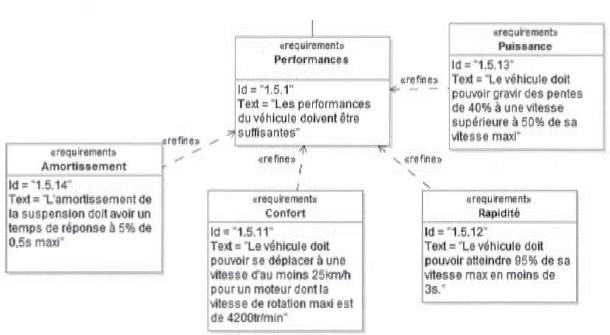
\includegraphics[width=.5\linewidth]{fig_02_bis}

\end{center}

\begin{center}
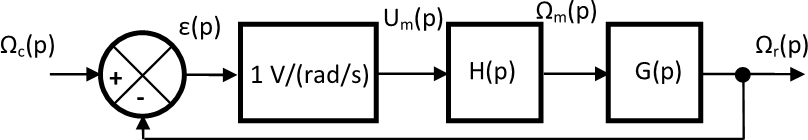
\includegraphics[width=.8\linewidth]{fig_03}

\textit{Figure 1 -- Hélicoptère.}
\end{center}


\begin{center}
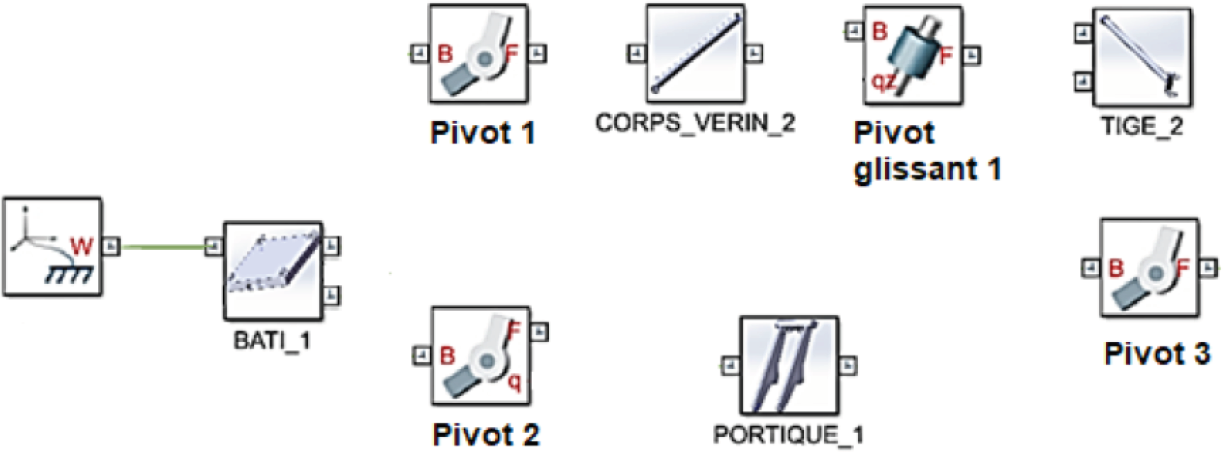
\includegraphics[width=.8\linewidth]{fig_04}

\textit{Figure 2 -- Structure du banc d'essai.}
\end{center}

\section*{Le moteur à courant continu}
Le banc d'essai est équipé d'un dispositif permettant de générer un couple résistant sur le rotor de sortie de la BTP. Cela permet de simuler les actions aérodynamiques sur les pales. Il faut donc évaluer l'impact de ce couple sur la vitesse du moteur. 
La modélisation adoptée pour le moteur à courant continu est celle de la figure 3.
 
\begin{center}
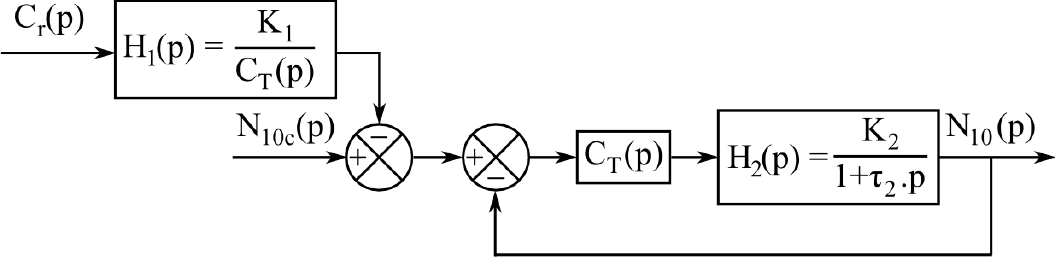
\includegraphics[width=.8\linewidth]{fig_05}

\textit{Figure 3 -- Schéma équivalent du moteur à courant continu.}
\end{center}



On note :
\begin{itemize}
	\item $u(t)$ : la tension appliquée aux bornes de l'induit ;
	\item $i(t)$ : le courant absorbé par l'induit ;
	\item $e(t)$ : la force contre-électromotrice ;
	\item $R$ : la résistance de l'induit ;
	\item $L$ : l'inductance de l'induit ;
	\item $\omega_m (t)$ : la vitesse de rotation de l'arbre moteur ;
	\item $c_m (t)$ : le couple moteur ;
	\item $c_r (t)$ : le couple résistant sur l'arbre moteur dû à la génération d'un couple résistant en sortie de BTP ;
	\item $f$ : le coefficient de frottement, qui génère un couple résistant proportionnel à $\omega_m (t)$ ;
	\item $I_{eq}$ : l'inertie équivalente du banc d'essai ramené à l'arbre moteur ;
	\item $K_c$ : la constante de couple définie telle que
 $c_m (t)=K_c i(t)$	(équation 1);
	\item $K_e$: la constante de force contre-électromotrice définie telle que $e(t)=K_e \omega_m (t)$	(équation 2).
	\end{itemize}
%	
Hypothèses :
\begin{itemize}
\item le comportement de chacun des composants sera considéré comme linéaire, continu et invariant ;
\item les conditions de Heaviside sont considérées comme vérifiées ;
\item on note $p$ la variable de Laplace. La transformée de Laplace d'une fonction temporelle $f(t)$ sera notée $F(p)$ (la transformée de $\omega(t)$ sera notée $\Omega(p)$).
\end{itemize}

%\subparagraph{}\textit{En justifiant, donner la relation électrique entre $e(t)$, $i(t)$ et $u(t)$.}
%
%On se réfère au schéma cinématique présenté figure 2. On note $I_i$ le moment d'inertie du 
%solide $i$ autour de l'axe de rotation du solide.
%
%\subparagraph{}\textit{Déterminer l'énergie cinétique $E_c (7⁄0)$ de l'ensemble 7 par rapport à 0 en fonction de $\omega(7⁄0)$ et de $I_7$ puis l'énergie cinétique $E_c (6⁄0)$ de l'ensemble 6 par rapport à 0 en fonction de $\omega(7⁄0)$, $Z_7$, $Z_6$ et $I_6$. En déduire l'énergie cinétique $E_c (((6+7))⁄0)$ ainsi que l'inertie équivalente aux solides 6 et 7 (notée $I_{67}$) ramenée sur l'arbre 7.}
%
%Par extension on pourrait déterminer l'inertie équivalente $I_{eq}$ de l'ensemble $E=\{1,2,3,4,5,6,7,BTP\}$ ramenée sur l'arbre moteur 7.
%\subparagraph{}\textit{En utilisant la figure 3 et par la méthode de votre choix, déterminer la relation entre $c_m (t)$, $c_r (t)$, $\omega_m (t)$, $\dfrac{d\omega_m (t)}{dt}$, $I_{eq}$ et $f$.}

%En utilisant le théorème du moment dynamique appliqué à l'arbre en rotation en un point de l'axe et en projection sur l'axe moteur (équation 3):
%$$
%c_m(t)-c_r(t)-f\omega_m(t) = I_{eq} \dfrac{\text{d} \omega_m(t)}{\text{d}t}.
%$$
%
%Enfin, $u(t)=L\dfrac{\text{d}i(t)}{\text{d}t}+Ri(t)+e(t)$ (équation 4).
%
%\subparagraph{}\textit{Traduire dans le domaine de Laplace les équations (1), (2), (3) et (4) . Réaliser alors le schéma bloc associé au moteur à courant continu.}
%
%\subparagraph{}\textit{On fait l'hypothèse que $c_r(t)=0$. Déterminer la fonction de transfert en boucle fermée $\dfrac{\Omega_m(p)}{U(p)}$. Déterminer les constantes caractéristiques d'un système d'ordre 2. }


%\subparagraph{}\textit{Donner la fonction de transfert du moteur et la mettre sous forme canonique en donnant l'expression littérale de chacune des constantes.}
\section*{Modélisation de l'asservissement en vitesse}
Hypothèses :
\begin{itemize}
\item on néglige l'inductance du moteur à courant continu ainsi que l'effet du coefficient de frottement ;
\item on fait l'hypothèse que $K_c=K_e =K$;
\item pour simplifier l'étude, la boucle de courant n'a pas été modélisée.
\end{itemize}
Le schéma bloc de l'asservissement en vitesse du moteur à courant continu est donné sur la figure 10.
 

\begin{center}
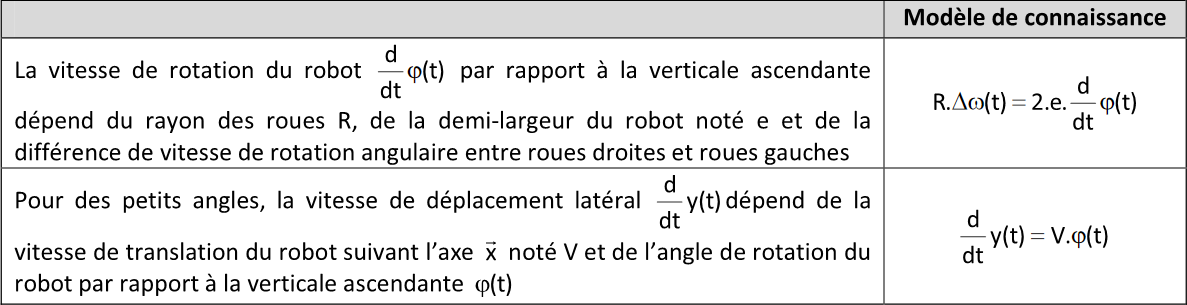
\includegraphics[width=\linewidth]{fig_06}

\textit{Figure 10 -- Régulation en vitesse du banc d'essai.}
\end{center}

\subparagraph{}\textit{Quelle solution technologique peut-on utiliser pour le capteur situé en boucle de retour ? Comment déterminer la valeur du gain $K_{\text{Adapt}}$ ?}

\subsection*{Hypothèse 1 : on considère que $C_r (p)=0$ et $\Omega_c (p)\neq 0$.}
\subparagraph{}\textit{Déterminer la fonction de transfert en boucle fermée $H_m (p)=(\Omega_m (p))/U(p)$ puis la fonction de transfert en boucle fermée $H_1 (p)=(\Omega_m (p))/(\Omega_C (p))$. On considère que $C(p)=K_P$, $K_P$ étant constant. Mettre $H_1 (p)$ sous la forme $K_1/(1+\tau_1 p)$ où on explicitera les valeurs de $K_1$ et $\tau_1$.}

\subsection*{Hypothèse 2 : on considère que $\Omega_C (p)=0$ et que $C_r (p)\neq0$.}
\subparagraph{}\textit{Retracer sur la copie le schéma bloc en tenant compte de ces hypothèses.}

\subparagraph{}\textit{Déterminer la fonction de transfert en boucle fermée $H_2 (p)=(\Omega_m (p))/(C_r (p))$. On considère que $C(p)=K_P$, $K_P$ étant constante. Mettre $H_2 (p)$ sous la forme $-K_2/(1+\tau_2 p)$ où on explicitera les valeurs de $K_2$ et $\tau_2$.}

\subsection*{Hypothèse 3 : on considère maintenant que  $\Omega_C (p)\neq 0$ et que $C_r (p)\neq 0$.}
\subparagraph{}\textit{En utilisant le théorème de superposition, exprimer $\Omega_m (p)$ en fonction de $H_1 (p)$, $H_2 (p)$, $\Omega_c (p)$ et $C_r (p)$.}

À une fréquence de rotation de $\SI{350}{min^{-1}}$ en sortie de BTP correspond une consigne de fréquence de rotation du moteur de $\SI{1 928}{min^{-1}}$ soit environ $\SI{202}{rad/s}$. Le couple résistant ramené à l'arbre moteur est évalué à $\SI{990}{Nm}$. On soumet donc le système à un échelon de consigne d'amplitude $\SI{202}{rad/s}$ et à un couple résistant de $\SI{990}{Nm}$.

\subparagraph{}\textit{Après avoir exprimé la consigne  $\Omega_c (p)$ puis le couple résistant $C_r (p)$, calculer sous forme littérale l'écart statique du système. Conclure vis-à-vis du cahier des charges.}
\subparagraph{}\textit{Quel intérêt peut présenter l'utilisation d'un correcteur intégral de gain $K_I$ de la forme $C(p)=K_I/p$ ?}
\subparagraph{}\textit{En conclusion, en utilisant le correcteur précédent, l'asservissement proposé permet-il de tenir la consigne de vitesse lorsqu'un couple résistant est appliqué à l'arbre de sortie de la BTP ? L'exigence 1.1.1 est-elle vérifiée ?}

\begin{rem}
On verra ultérieurement qu'un correcteur intégral pur ne permet pas forcément de garantir la stabilité d'un système.
\end{rem}
\section*{Partie supplémentaire}
\subparagraph{}\textit{Tracer le diagramme de Bode de $C(p)\cdot F(p)$ avec $F(p)=118/(1+0,5 p)$ du système lorsque : 
\begin{itemize}
\item $C(p)=1$;
\item $C(p)=20$ ;
\item $C(p)=30/p$.
\end{itemize}}

\end{multicols}
